\documentclass[a4paper, 12pt]{article}
\usepackage[left=2cm, right=2cm, top=2cm, bottom=2cm]{geometry}
\setlength{\parindent}{0cm}
\usepackage{graphicx}
\begin{document}
\title{My first LaTex document}
\author{Abheshek Kamble}
\date{\today}
\maketitle

\tableofcontents
\listoffigures

\section{Itroduction}

This is my submission for the assignment 4 for MM2090 course.
% This is a comment to helo me keep things sorted.


\section{Abheshek(me20b005)}
This is the equation I have chosen.
\begin{equation}
	k = Ae^{-E_a/RT}
	\label{eqn:arrhenius}
\end{equation}

It can also be written as
\begin{equation}
	\ln{k} = -E_a/RT + \ln{A}
	\label{eqn2:arrhenius}	
\end{equation}

\begin{figure}[h]
	\begin{center}
		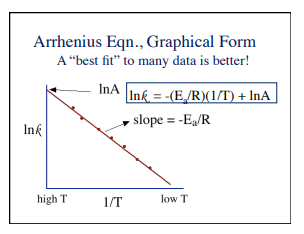
\includegraphics[scale=0.75]{arrhenius.png}
	\end{center}
	\caption{ME20B005}
	\label{f1:graph}
\end{figure}

The Arrhenius equation~\ref{eqn:arrhenius}~\ref{eqn2:arrhenius} gives the dependence of the rate constant of a chemical reaction on the absolute temperature where 
\begin{itemize}
	\item $k$ is the rate constant (frequency of collisions resulting in a reaction)
	\item $T$ is the absolute temperature (in kelvins)
	\item $A$ is the pre-exponential factor, a constant for each chemical reaction.The units of the pre-exponential factor A are identical to those of the rate constant and will vary depending on the order of the reaction. For a first-order reaction, it has units of $s^{-1}$. For that reason, it is often called frequency factor.According to collision theory, the frequency factor, A, depends on how often molecules collide when all concentrations are 1 $mol/L$ and on whether the molecules are properly oriented when they collide.
	\item $E_a$ is the activation energy for the reaction (in the same units as kBT).Activation energy can be thought of as the magnitude of the potential barrier (sometimes called the energy barrier) separating minima of the potential energy surface pertaining to the initial and final thermodynamic state. For a chemical reaction to proceed at a reasonable rate, the temperature of the system should be high enough such that there exists an appreciable number of molecules with translational energy equal to or greater than the activation energy.
	\item R is the universal gas constant

\end{itemize}

This equation has a vast and important application in determining rate of chemical reactions and for calculation of energy of activation~\cite{bohn}

In figure~\ref{f1:graph} we can see the relation of $\ln{k}$ and $1/T$ and also see the $y$ intercept. From this graph, at a given temperature we can find the value of rate constant for a reaction~\cite{fabrikant}.




\bibliography{citation}
\bibliographystyle{plain}



\end{document}